\documentclass[11pt]{article}
\usepackage[a4paper,margin=2.5cm]{geometry}
\usepackage{amsmath,amssymb,amsthm}
\usepackage{graphicx}
\usepackage{booktabs}
\usepackage{enumitem}
\usepackage[hidelinks]{hyperref}
\usepackage{xcolor}
\usepackage{tikz}
\usetikzlibrary{arrows.meta,positioning}

\newtheorem{theorem}{Theorem}
\newtheorem{lemma}[theorem]{Lemma}
\newtheorem{proposition}[theorem]{Proposition}
\newtheorem{corollary}[theorem]{Corollary}
\theoremstyle{definition}
\newtheorem{definition}[theorem]{Definition}
\theoremstyle{remark}
\newtheorem{remark}[theorem]{Remark}
\newcommand{\Lam}{\Lambda}
\newcommand{\status}[1]{\textsf{\small[#1]}}

\title{The Kobon triangle problem for 18 lines:\\
an upper bound of 94 for all arrangements,\\
and a reduction of $K(18)=93$ to a single local configuration}
\author{Raj Harshit Srirangam\thanks{Computer-assisted work. The AI systems and compute that were used are disclosed in Section~\ref{sec:disclosure}.}}
\date{2 October 2026 \\ \small Preprint. Computer-assisted proofs; no human refereeing or formal verification yet.}

\begin{document}
\maketitle

\begin{abstract}
The Kobon triangle problem asks for the largest number $K(n)$ of bounded triangular faces in an arrangement of $n$
lines in the plane. For $n=18$ the best known arrangements have $93$ triangles.
\begin{itemize}[nosep]
\item For \emph{simple} arrangements (no three lines through a point) Blanc proved $93$ is optimal.
\item For arrangements with multiple points, the best bounds previously known to us are Tamura's $96$ and an
unpublished $95$.
\end{itemize}
We prove, with computer assistance, that \textbf{every arrangement of $18$ lines or pseudolines, of any
multiplicity, has at most $94$ bounded triangles}. We also prove that an arrangement with $94$ triangles cannot
have multiplicity at most three. We further show that a vertex-maximal $94$ contains only triple points and
``bad'' fourfold points, and must contain a fourfold point all eight of whose angles are triangles (an
\emph{all-8 point}).

The proofs combine three ingredients:
\begin{itemize}[nosep]
\item an exact budget identity, $\Lam = 18\cdot 16-3T = Z+\sum_P c_P$;
\item a generalisation of the Bartholdi--Blanc--Loisel charging argument, made rigorous by per-line linear-programming
certificates. These are checked exactly by dynamic programming over a finite automaton describing every possible line;
\item local optimality lemmas, proved by exhaustive enumeration of local redrawings.
\end{itemize}
The same certificates hold at other $n$. They prove $K(14)=54$ for \emph{all} arrangements, a new exact value. For
multiplicity at most three they prove the Bartholdi--Blanc--Loisel bound $\lfloor n(n-7/3)/3\rfloor$ for every even $n$
from $6$ to $40$, which gives $K(16)=72$ and $K(20)=117$ in that class; previously these bounds were proved only for
simple arrangements.
For the remaining all-8 case we prove an exact identity
$\Lam=\pi+U+\tfrac12\sum_P S^\circ_P+K_3+2K_4+\tfrac12\Delta$ with all terms nonnegative; $K(18)=93$ is equivalent
to $\Lam\ge 7$ in this case, which is open. We release exact arrangements, triangle certificates, an independent checker,
and all proof certificates with verification commands.
\end{abstract}

\section{Introduction}

Let $\mathcal A$ be an arrangement of $n$ lines in the Euclidean plane and $T(\mathcal A)$ the number of its bounded
faces that are triangles, i.e.\ nondegenerate triangles not crossed by any line. The Kobon triangle problem, posed
by Kobon Fujimura, asks for $K(n)=\max T(\mathcal A)$.

The classical upper bound is Tamura's $K(n)\le\lfloor n(n-2)/3\rfloor$: each of the $n(n-2)$ bounded segments of a
simple arrangement borders at most two triangles, and the extremal configurations are restricted further. Clément and
Bader~\cite{clementbader} sharpened it by one for $n\equiv 0,2\pmod 6$. Bartholdi, Blanc and Loisel~\cite{bbl} proved
$T\le\lfloor n(n-7/3)/3\rfloor$ for \emph{simple} arrangements of lines and pseudolines; this is the source of the
value $94$ for $n=18$ that is often quoted. Blanc~\cite{blanc} improved this to $\lfloor n(n-5/2)/3\rfloor$ for even
$n$, which is $93$ at $n=18$. Both papers state and use simplicity.

For arrangements with points of multiplicity at least three, which occur in every known record for even $n$, we are
not aware of a bound at $n=18$ better than $96$ (Tamura) or the unpublished $95$~\cite{clementbader}. The best known
construction has $93$ triangles~\cite{gallery}. So, before this work, $K(18)$ was known only to lie in $\{93,94,95,96\}$
(or $\{93,94,95\}$ if~\cite{clementbader} is accepted).

\paragraph{Results.} All results below concern arrangements of $n=18$ pseudolines (each pair crossing exactly once);
straight-line arrangements, including parallel lines, are covered by the standard projective treatment of parallel
classes. ``Computer-assisted'' means that the proof reduces to exact computations whose certificates we publish.

\begin{theorem}[computer-assisted]\label{thm:94}
Every arrangement of $18$ pseudolines has at most $94$ bounded triangles.
\end{theorem}

\begin{theorem}[computer-assisted]\label{thm:mult3}
Every arrangement of $18$ pseudolines in which no point lies on four or more lines has at most $93$ bounded triangles.
\end{theorem}

\begin{theorem}[computer-assisted]\label{thm:structure}
Let $\mathcal A$ be an arrangement of $18$ pseudolines with $94$ bounded triangles, chosen with the maximum number of
vertices. Then:
\begin{enumerate}[nosep,label=(\alph*)]
\item every multiple point of $\mathcal A$ is a triple point or a fourfold point whose cyclic word of eight sector
types (triangle $=1$) is, up to symmetry, $11111111$, $11111110$ or $11101110$;
\item there is no point of type $11101110$;
\item there is a point of type $11111111$ (an \emph{all-8 point});
\item some fourfold point and some triple point are consecutive on a line, and every such consecutive pair has one of
$48$ explicitly listed local patterns;
\item every triple point has both alternating sums of its six sector bits at least $2$.
\end{enumerate}
\end{theorem}

Theorems~\ref{thm:94}--\ref{thm:structure} reduce the question $K(18)=93$ to excluding arrangements with an all-8
point. We do not complete this exclusion. Section~\ref{sec:open} gives the sharpest reduction we have: an exact
identity in nonnegative local credits. We also explain why the per-line method that proves
Theorem~\ref{thm:94} cannot finish the job as it stands.

On the construction side we found, by our own unseeded search, a new straight-line $18$-line arrangement with $93$
triangles and no multiple points. It is scored $93$ by the competition's exact evaluator, and $93$ ties the record.
It is \emph{not} a new record.

\paragraph{Status.} The proofs were developed with AI assistance (Section~\ref{sec:disclosure}). They have been checked
by exact computation, by independent reimplementations and by an independent audit, but not by a human referee or a
proof assistant. Table~\ref{tab:status} lists each claim with its evidence.

\section{Preliminaries: the budget identity}

Fix an arrangement $\mathcal A$ of $n$ pseudolines. A \emph{segment} is a bounded edge, i.e.\ a piece of a line
between consecutive vertices. A segment is \emph{used} by each triangle having it as a side, so it is used $0$, $1$
or $2$ times. Let $Z$ be the number of unused segments. For a point $P$ of multiplicity $m_P\ge 3$ let:
\begin{itemize}[nosep]
\item $D_P$ be the number of rays at $P$ whose first segment is used twice and ends at a simple vertex (\emph{blocks});
\item $\beta_P$ be the number of such rays ending at a multiple point (\emph{bridges});
\item $N_P=2m_P-D_P-\beta_P$ be the number of remaining rays.
\end{itemize}

\begin{lemma}[budget identity]\label{lem:budget}
With $\Lam=n(n-2)-3T$,
\[
\Lam = Z+\sum_{m_P\ge 3}c_P,\qquad c_P=m_P(m_P-2)-D_P-\tfrac12\beta_P .
\]
For triple points $c_P=(N_P-D_P)/2$, and for fourfold points $c_P=4+(N_P-D_P)/2$. For $n=18$, $\Lam=288-3T$ is
divisible by $3$; thus $T=94\iff\Lam=6$, and $T\le 93\iff\Lam\ge 7$.
\end{lemma}
\begin{proof}[Proof sketch]
Count triangle sides: $3T=(S-Z)+D_2$, where $S$ is the number of segments and $D_2$ the number of segments used twice.
A doubly used segment always has a multiple endpoint (L1): two triangles on both sides of a segment between two simple
vertices would force a second crossing. Hence $D_2=\sum_P D_P+\tfrac12\sum_P\beta_P$. Finally,
$S=n(n-2)-\sum_P m_P(m_P-2)$, since each line through a point of multiplicity $m$ loses $m-2$ vertices.
\end{proof}

\paragraph{Per-line form.} Splitting $3c_P$ over the rays at $P$ ($+\tfrac32$ per $N$ ray, $-\tfrac32$ per block, $0$ per
bridge), and splitting each unused segment into three \emph{portions}, gives
\[
3\Lam-n=\sum_L v_L+\mathrm{waste},\qquad \mathrm{waste}\ge 0 .
\]
One portion goes to its own line and one to the other line at each simple endpoint. $v_L$ depends only on the line
$L$ and the faces incident to it. This is the per-line form of the Bartholdi--Blanc--Loisel argument~\cite{bbl}: in a
simple arrangement with $n$ even, every line has $v_L\ge 0$, which gives $\Lam\ge n/3$. With multiple points individual
lines can be negative, and charge must be moved between lines by \emph{transfer rules}.

\section{Per-line certificates}\label{sec:cert}

\paragraph{Transfer rules and the line automaton.} We fix a finite catalogue of local \emph{cells}: configurations
around a block, a simple vertex, a triangle, or a multiple point that are visible from every line taking part. Each
cell carries a transfer between the lines involved, with a weight $w$; the transfers cancel exactly, so for every $w$
\[
3\Lam-18=\sum_L \mathrm{final}_L(w)+\mathrm{waste}.
\]
To bound $\mathrm{final}_L$ from below for \emph{every} line of every arrangement, we encode the view from a single
line as a word over a finite alphabet of \emph{frames}. A frame records the vertex type (simple, triple, fourfold),
the triangle bits on both sides of the adjacent segments, and the multiplicity classes of triangle apexes. Hidden
sector bits are also recorded, together with local facts that we prove separately. A line with $17$ crossings is a
path of exact weight $17$ in a layered graph. $\mathrm{final}_L$ is a sum of window terms along the path, so
$\min_L\mathrm{final}_L$ is a shortest-path computation, i.e.\ a dynamic program (DP).

\paragraph{Certificates.} A cutting-plane loop alternates between a linear program over the weights, the DP (which
returns the worst path), and, where needed, SAT checks that a candidate worst path is not realisable. Proved
unrealisable patterns are added to the automaton. The final weights are rationalised to a common denominator $D$,
and the DP is rerun in exact integer arithmetic.

\begin{proposition}[certificate FC]\label{prop:fc}
For multiplicity $\le 3$ there are weights with $D=16$ such that every automaton path has
$\mathrm{final}\ge 0$. Hence $\Lam\ge 6$, i.e.\ $T\le 94$.
\end{proposition}

\begin{proposition}[certificate FC-M]\label{prop:fcm}
For arbitrary multiplicity, with fourfold points restricted to the three bad words of
Theorem~\ref{thm:structure}(a) (Lemma~\ref{lem:pert}) and the pair lemma (Lemma~\ref{lem:pair}), there are weights
with $D=16$ such that every path has $\mathrm{final}\ge -\tfrac14$. Hence $3\Lam-18\ge -18/4>-9$. Since $3\Lam-18$ is
a multiple of $9$, $3\Lam-18\ge 0$, i.e.\ $\Lam\ge 6$.
\end{proposition}

Propositions~\ref{prop:fc} and~\ref{prop:fcm}, with the reduction of Lemma~\ref{lem:pert}, prove
Theorem~\ref{thm:94}. The automaton facts used by the certificates were validated on several million real lines: no
real line violates a fact, and the exact DP minimum is reproduced by an independent second DP.

\section{Local optimality lemmas}\label{sec:local}

If an arrangement with $T=94$ exists, choose one with the maximum number of vertices. Redrawing a small disk around a
point, with the same boundary crossings, gives another pseudoline arrangement. The redrawing can neither increase $T$
(Theorem~\ref{thm:94}), nor keep $T$ while increasing the number of vertices.

\begin{lemma}[perturbation lemma]\label{lem:pert}
In a vertex-maximal $94$, every point of multiplicity $\ge 4$ is a fourfold point with sector word $11111111$,
$11111110$ or $11101110$, up to symmetry.
\end{lemma}
\noindent The local redrawings are enumerated exhaustively for multiplicities $4$ and $5$; for $6$ they come from a sampled
covering set; for $7\le m\le 17$ there are explicit lossless simple redrawings. The enumeration was re-derived with an
independent face computation by half-edge tracing (1,945 local words, 0 mismatches).

\begin{lemma}[pair lemma]\label{lem:pair}
In a vertex-maximal $94$, if a fourfold point $P$ and a triple point $Q$ are consecutive on a line, then the pair of
sector words of $(P,Q)$ is one of $48$ canonical patterns (out of $2{,}080$). For an all-8 point $P$, the triple
neighbour's word is one of $100111$, $101101$, $101111$, $110011$, $110111$, $111111$.
\end{lemma}

\begin{lemma}[triple optimality]\label{lem:triopt}
In a vertex-maximal $94$, every triple point with sector bits $s_0,\dots,s_5$ satisfies $s_0+s_2+s_4\ge 2$ and
$s_1+s_3+s_5\ge 2$.
\end{lemma}
\begin{proof}
Resolving a triple point into three simple crossings creates one small triangle. It adds one side to each sector of one
alternating triple, so $\Delta T=1-(s_0+s_2+s_4)$ or $1-(s_1+s_3+s_5)$, while the vertex count grows by $2$.
\end{proof}

\section{Excluding cases}\label{sec:excl}

\paragraph{Multiplicity at most three (Theorem~\ref{thm:mult3}).} In a $94$ we have $3\Lam-18=0$. So under every
certificate with $\varepsilon=0$, every line is \emph{exactly} tight and the waste is zero. Intersecting the tight
sets of five certificates (joint tightness) and iterating an exact elimination shows the following:
\begin{itemize}[nosep]
\item there are no unused segments;
\item only four point types survive;
\item via a Gauss--Bonnet count on the bridge components, there are three structural cases: six isolated ``X'' points,
one seven-point ``flower'' plus three X points, or two flowers.
\end{itemize}
The flower cases are closed by a tip lemma: two end conditions at opposite tips are jointly unsatisfiable among nine
pseudolines, with a DRAT-certified SAT proof. The six-X case is closed by an independent cube SAT computation
(2,841 cubes, all DRAT-verified). This chain was audited independently (five items, all passed).

\paragraph{Fourfold points.} With fourfold points present, certificates with an extra \emph{credit} at a fourfold point
of a given word show $\sum_L\mathrm{final}_L>0$, contradicting $3\Lam-18=0$:
\begin{itemize}[nosep]
\item word $11101110$: margin $9/8$ (Theorem~\ref{thm:structure}(b));
\item word $11111110$, when no all-8 point is present: margin $7/10$;
\item a strict certificate shows some fourfold--triple adjacency is necessary (Theorem~\ref{thm:structure}(d)).
\end{itemize}
Together with Theorem~\ref{thm:mult3} and Lemma~\ref{lem:pert}, a $94$ must contain an all-8 point
(Theorem~\ref{thm:structure}(c)).

\section{The remaining case: an all-8 point}\label{sec:open}

\paragraph{Why the per-line method stops.} For the all-8 case, the best per-line credit LP we could build has margin
$-2.29$ instead of a positive one. This value is unchanged by every refinement we tried: hidden state along the line,
further proved lemmas, the triple optimality filter, sixteen SAT-proved local patterns, and new kite-transfer rules.
More decisively, SAT realises the binding paths as \emph{actual} lines of arrangements in the class (29 of the 61 binding paths; 31 timed out
and one was unrealisable). In those arrangements the line through the all-8 point is at the floor,
while the other lines through the same point carry large surplus. Per-line accounting with local rules cannot move
credit between the lines of a star.

\paragraph{A two-dimensional credit identity.} Classify the blocks at their simple endpoint $X$: \emph{touch} ($U$: the
continuation beyond $X$ is bounded and unused), \emph{end} ($I$: the line ends at $X$), or \emph{mutual}. Mutual blocks
meet at a $3$-fan or at a \emph{kite} (a simple vertex with four triangles). Let $K_q$ be the number of kites with
exactly $q$ fourfold corners.

Injective payments assign to every block a token: an $N$ ray on a singly used segment, identified by its unique
triangle. They give the following.
\begin{itemize}[nosep]
\item No two consecutive blocks at a triple point, and no three at a fourfold point.
\item Every kite with four triple corners has a singly used cap edge in each pair of opposite sides.
\item Every kite with exactly one fourfold corner is paid. Either one of its cap edges is singly used, or its fourfold
corner has slack two by a far-corner argument.
\item Every touch or end block from a fourfold point receives a fresh token.
\end{itemize}

Consider the line ends next. Call an end of line $L$ at the simple vertex $v=L\cap M$ a \emph{bad wedge} if $v$ is also
the last vertex of $M$ and the bounded face opposite the wedge is a triangle. Join two lines when they meet at a bad
wedge.

\begin{lemma}[forest lemma]
For $n$ even, the bad-wedge graph is a forest of paths; let $\pi\ge 1$ be its number of components.
\end{lemma}
\begin{proof}[Proof sketch]
If both ends of $L$ are bad wedges, the two corner triangles lie on the same side of $L$. A cycle of $k$ lines then
forces $k$ odd, by counting crossings of the closed curve with one of its lines. Any line outside the cycle crosses
the curve $k$ times, which forces $k$ even. So a cycle must contain every line, and $n$ is odd.
\end{proof}

\begin{theorem}[credit identity]\label{thm:identity}
For $18$ pseudolines in the class of Theorem~\ref{thm:structure},
\[
\Lam=\pi+U+\tfrac12\sum_P S^\circ_P+K_3+2K_4+\tfrac12\Delta,
\]
every term $\ge 0$. Here:
\begin{itemize}[nosep]
\item $S^\circ_P=8-D_P-k_P-2c_B(P)$ is the corrected slack at a fourfold point, where $k_P$ counts its blocks ending at
kites and $c_B(P)$ its kites with all cap edges doubly used;
\item $\Delta\ge 0$ counts unused end slots and unused tokens.
\end{itemize}
\end{theorem}

\noindent So a $94$ needs $\pi+U+K_3+2K_4\le 6$, i.e.\ at least $12$ bad wedges, and $K(18)=93$ is equivalent to
\[
2\pi+2U+\textstyle\sum_P S^\circ_P+2K_3+4K_4+\Delta\ \ge\ 13
\]
for this class. For simple arrangements, the forest lemma and the parity lemma below already give Blanc's case
$\Lam\ge 6$ in a few lines. Every line with both ends bad must contain an unused segment, so
$\Lam\ge\max(\pi,18-2\pi)\ge 6$.

\begin{lemma}[parity]
Let $L$ have all bounded segments singly used and both ends bad wedges. Let $t_L$ be the number of triple points on
$L$, and $f_L$ the number of touch or end centres capped by $L$. If $n$ is even, $t_L+f_L$ is odd.
\end{lemma}

\paragraph{What is missing.} The known $93$s spread their $\Lam=9$ over all terms. Among $14{,}376$ of them,
$(\pi,U,\tfrac12\Delta)$ ranges from $(9,0,0)$ to $(1,0,8)$ and $(2,7,0)$. So no single term can be forced. What is
needed is a trade-off lemma in the class: many bad wedges force parity defects on the lines between them, and these
defects force $U$ or $\Delta$. Lines through triple points flip parity at no cost, and this is the core difficulty.
Partial results toward a two-stage finish: (B) $E\ge 18-3\pi$ would force a $94$ into the zero-credit corner
$\pi=6$, $E=0$. In that corner, hand counts of the lines forced by local saturation exclude every cluster of
fourfold points except two local types. These are an isolated double-case-B star (at least $14$ lines) and a
two-point path with two case-B ends (at least $17$ lines). The proof of (B) is reduced to a local capacity inequality
that holds on all known data. Small cases are also decided by SAT: with an all-8 point in
the class, $\Lam\le 6$ is impossible for $n\le 10$, and the minimum is $\Lam=9$ at $n=9$ and $8$ at $n=10$.

\section{Constructions}\label{sec:constr}

Figure~\ref{fig:93} shows two $18$-line arrangements with $93$ triangles:
\begin{itemize}[nosep]
\item our arrangement, found by unseeded simulated annealing over line angles and offsets with a fast floating-point
counter, then rounded to integer coefficients and recounted exactly. It has no multiple points;
\item an arrangement with three triple points from the Utkin--Parpalak gallery~\cite{gallery}.
\end{itemize}
Both are counted by the competition evaluator and by our independent checker (Section~\ref{sec:verify}), with
identical triangle sets. The frozen baseline of the competition, $18$ tangents to a parabola, has $16$ triangles. For
$n=15$ we also obtained the proven optimum $65$ by the same search. Searches for a $94$ found none:
\begin{itemize}[nosep]
\item exact one-line extensions of all $255$ perfect $17$-line wiring diagrams;
\item re-insertion of every line of $3{,}016$ known $93$s;
\item $4$-line merges of $42{,}331$ arrangements with $T\ge 92$;
\item SAT searches in many structured families.
\end{itemize}

\begin{figure}[t]
\centering
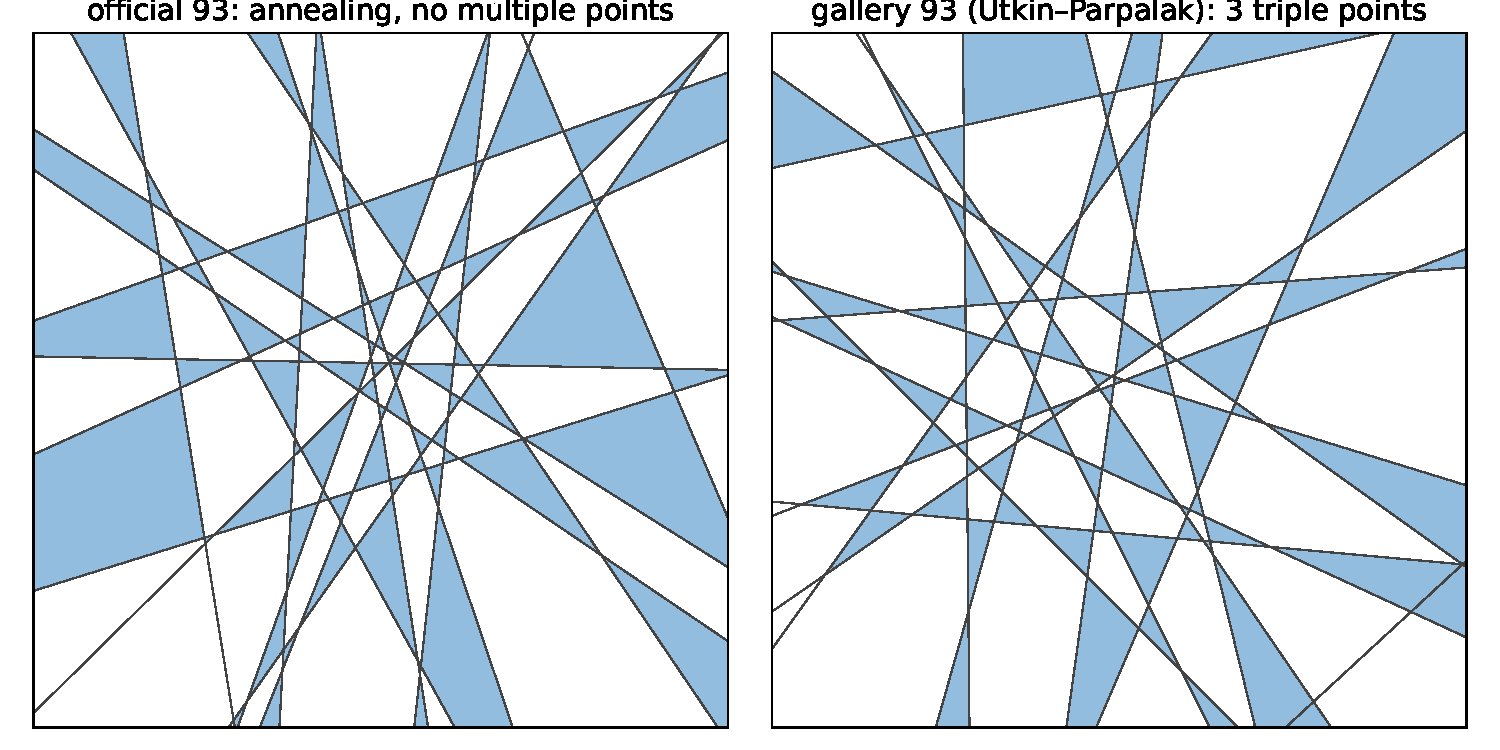
\includegraphics[width=\textwidth]{figures/two93.pdf}
\caption{Two arrangements of $18$ lines with $93$ bounded triangles (shaded), central region. Some long thin triangles
extend beyond the frame. Left: our arrangement (no multiple points), scored $93$ by the exact evaluator. Right: an
arrangement from~\cite{gallery} with three triple points. Exact coefficients and triangle lists are in
\texttt{arrangements/}.}
\label{fig:93}
\end{figure}

\section{Further results for general $n$}\label{sec:general}

\begin{theorem}[computer-assisted]\label{thm:othern}
\begin{enumerate}[nosep,label=(\alph*)]
\item For every even $n$ with $6\le n\le 40$, every arrangement of $n$ pseudolines with no point on four or more lines
has $T\le\lfloor n(n-7/3)/3\rfloor$. This equals the known record at $n=6,8,10,12,14,16,20$~\cite{gallery,oeis}. So in
this class $K(n)$ is determined for these $n$, and in particular $K(16)=72$ and $K(20)=117$.
\item Every arrangement of $14$ lines or pseudolines, of any multiplicity, has $T\le 54$. Hence $K(14)=54$.
\end{enumerate}
\end{theorem}
\begin{proof}[Proof sketch]
(a) Take the certificate FC of Proposition~\ref{prop:fc}, with unchanged weights. Its ingredients are valid for all
$n$: the automaton facts, the cell domains (an enumeration over automaton windows, filtered by local facts with hand
proofs), and the base identity. Only the exact path weight $W=n-1$ changes. Rebuilding the automaton for each even
$n\le 40$ and rerunning the exact DP gives $\min\mathrm{final}=0$. Hence $3\Lam-n\ge 0$, and with
$\Lam\equiv n(n-2)\pmod 3$ the bound follows.

(b) The certificate FC-M of Proposition~\ref{prop:fcm} verifies at $W=13$ with $\min\mathrm{final}\ge-\tfrac14$. Its
SAT-proved local patterns, which were proved for $18$ lines, were re-proved for $14$ lines with DRAT certificates. The
perturbation and pair lemmas are local. Then $3\Lam-14\ge-\tfrac{14}{4}>-5$. Since $\Lam\equiv 0\pmod 3$ and
$3\cdot 3-14=-5$, we get $\Lam\ge 6$, i.e.\ $T\le 54$.
\end{proof}
\noindent The records at $n=14$ and $n=20$ use triple points and exceed Blanc's bounds for simple arrangements ($53$
and $116$), so the simple-arrangement theorems did not settle these values.

Two further results from the same framework hold for every even $n$. Their certificates and proofs are in the
repository.
\begin{theorem}[Theorem G]
Let $n$ be even and let $\mathcal A$ be an arrangement of $n$ lines or pseudolines (no three lines mutually parallel)
with $t$ triple points and no line
through two multiple points. Then $\Lam\ge n/2-t$, i.e.\ $T\le\lfloor(2n^2-5n+2t)/6\rfloor$. For $t=0$ this is Blanc's
bound.
\end{theorem}
\begin{theorem}[automaton-certified, all even $n$]
For arrangements with only simple and triple points whose triple points belong to one of three restricted classes of
local types, every line has $\mathrm{final}\ge 0$ under explicit transfer rules. Hence $\Lam\ge n/3$; for example
$T\le 54$ at $n=14$ and $T\le 72$ at $n=16$.
\end{theorem}
\noindent The second theorem is certified by an automaton without a length bound, so the certificate covers all $n$
at once. Theorem G has a hand proof that was checked by an independent AI referee.

\section{Verification and limitations}\label{sec:verify}

\begin{table}[t]
\centering\small
\begin{tabular}{p{4.6cm}p{6.4cm}p{3.2cm}}
\toprule
Claim & Evidence & Status \\
\midrule
Thm.~\ref{thm:94}, mult.\ $\le 3$ & exact certificate FC ($D=16$), DP rerun exactly; second DP & computer-verified \\
Thm.~\ref{thm:94}, fourfold points & exact certificate FC-M ($D=16$, $\varepsilon=\tfrac14$) & computer-verified \\
Thm.~\ref{thm:mult3} & joint tightness, elimination, ILP; tip lemma (DRAT); 6-X case (2,841 DRAT cubes) & computer-verified, audited \\
Lemma~\ref{lem:pert}, \ref{lem:pair} & exhaustive enumeration; independent re-derivation & computer-verified \\
Thm.~\ref{thm:structure}(b), (d), and the 7-type case & exact credit certificates & computer-verified \\
Thm.~\ref{thm:othern}(a) & certificate FC rechecked exactly at $W=n-1$, even $n\le 40$ & computer-verified \\
Thm.~\ref{thm:othern}(b), $K(14)=54$ & certificate FC-M at $W=13$; patterns re-proved for $14$ lines (DRAT) & computer-verified \\
Thm.~\ref{thm:identity} and lemmas of \S\ref{sec:open} & hand proofs, each checked; exact checks on $3{,}474$ arrangements & proofs checked, not refereed \\
$K(18)=93$ & --- & \textbf{open} (all-8 case) \\
\bottomrule
\end{tabular}
\caption{Claims and evidence. ``Computer-verified'' means an exact rational or SAT/DRAT certificate that can be rechecked
with the published scripts.}
\label{tab:status}
\end{table}

\paragraph{Independent checks.}
\begin{itemize}[nosep]
\item Triangle counts are verified by a standalone exact checker (rational arithmetic, two independent methods:
half-edge face enumeration and a triple test against every other line).
\item The perturbation and pair lemmas were re-derived with an independent half-edge face computation.
\item The multiplicity-$\le 3$ chain was audited independently, with two independent encodings of the tip lemma.
\item Every SAT exclusion used in a proof has a DRAT proof checked by \texttt{drat-trim}.
\end{itemize}

\paragraph{Limitations.}
\begin{enumerate}[nosep]
\item No human refereeing and no formalisation (no Lean or other proof assistant).
\item The automaton facts (``guarded facts'') used at fourfold apexes are validated on large real data sets, but their
hand proofs are not all written out. (The two special-column identities used by the fourfold certificates, previously
only validated on data, are now proved for every multiplicity; see the repository.)
\item The independent audit covers the multiplicity-$\le 3$ chain only, not the fourfold certificates.
\item SAT encodings are validated on many pinned cases but not formally verified.
\item The main open case is stated in Section~\ref{sec:open}.
\end{enumerate}

\section{Reproducibility}
All files are in the accompanying repository:
\begin{itemize}[nosep]
\item exact arrangements with triangle certificates: \texttt{arrangements/};
\item the independent checker: \texttt{checker/};
\item proof certificates with verification commands, expected outputs and logs: \texttt{certificates/};
\item the code and data they need: \texttt{search/}, \texttt{work/}, \texttt{tools/} (layout kept so that every
command runs unchanged);
\item technical notes, including the full proofs of the lemmas in Section~\ref{sec:open}: \texttt{proofs/};
\item a catalogue of $14{,}376$ distinct $93$-triangle $18$-pseudoline arrangements (wiring words, $0$ to $21$ triple
points): \texttt{data/}.
\end{itemize}
Dependencies are pinned in \texttt{requirements.txt}; \texttt{REPRODUCE.md} lists every command.

\section{Disclosure}\label{sec:disclosure}
This work was carried out with AI systems:
\begin{itemize}[nosep]
\item Claude Opus 5.5 (Anthropic), in Claude Code, did the planning, the mathematics and the checking of all proofs;
\item Claude Sonnet 5.5 subagents wrote software and performed audits;
\item GPT~6.1 contributed the notes behind the credit identity of Section~\ref{sec:open} (forest lemma, injective
payments). Every step was checked before use.
\end{itemize}
Computation ran on one 24-core workstation (62\,GB RAM). The construction was scored on the AutoLab platform
(competition hill \texttt{alejandrozu/kobon-triangles}, official report \texttt{203bd68f}, $93$ triangles at $n=18$).
The author directed the work and takes responsibility for the claims.

\begin{thebibliography}{9}
\bibitem{bbl} N.~Bartholdi, J.~Blanc, S.~Loisel, \emph{On simple arrangements of lines and pseudo-lines in
$\mathbb P^2$ and $\mathbb R^2$ with the maximum number of triangles}, arXiv:0706.0723 (2007).
\bibitem{blanc} J.~Blanc, \emph{The best polynomial bounds for the number of triangles in a simple arrangement of $n$
pseudo-lines}, arXiv:0801.2845 (2008).
\bibitem{clementbader} G.~Clément, J.~Bader, \emph{Tighter upper bound for the number of Kobon triangles}, unpublished
draft (2007).
\bibitem{gallery} A.~Utkin, R.~Parpalak, online gallery of Kobon triangle arrangements, \url{https://parpalak.com}
(accessed September 2026).
\bibitem{oeis} OEIS Foundation, \emph{Sequence A006066 (Kobon triangle numbers)}, \url{https://oeis.org/A006066}.
\end{thebibliography}
\end{document}
